\PassOptionsToPackage{no-math,cm-default}{fontspec}
\documentclass[twoside,nofonts,internet,shmeiwseis]{thewria}
\usepackage{amsmath}
\usepackage{xgreek}
\let\hbar\relax
\defaultfontfeatures{Mapping=tex-text,Scale=MatchLowercase}
\setmainfont[Mapping=tex-text,Numbers=Lining,Scale=1.0,BoldFont={Minion Pro Bold}]{Minion Pro}
\newfontfamily\scfont{GFS Artemisia}
\font\icon = "Webdings"
\usepackage[amsbb]{mtpro2}
\usepackage{tikz,pgfplots,tkz-euclide}
\tkzSetUpPoint[size=7,fill=white]
\xroma{red!80!black}


\newlist{rlist}{enumerate}{3}
\setlist[rlist]{itemsep=0mm,label=\roman*.}
\newlist{brlist}{enumerate}{3}
\setlist[brlist]{itemsep=0mm,label=\bf\roman*.}
\newcommand{\tss}[1]{\textsuperscript{#1}}
\newcommand{\tssL}[1]{\MakeLowercase{\textsuperscript{#1}}}
\usepackage{hhline}
%----------- ΓΡΑΦΙΚΕΣ ΠΑΡΑΣΤΑΣΕΙΣ ---------
\pgfkeys{/pgfplots/aks_on/.style={axis lines=center,
xlabel style={at={(current axis.right of origin)},xshift=1.5ex, anchor=center},
ylabel style={at={(current axis.above origin)},yshift=1.5ex, anchor=center}}}
\pgfkeys{/pgfplots/grafikh parastash/.style={\xrwma,line width=.4mm,samples=200}}
\pgfkeys{/pgfplots/belh ar/.style={tick label style={font=\scriptsize},axis line style={-latex}}}
%-----------------------------------------
\usepackage{multicol}
\usepackage{wrap-rl}
\tkzSetUpPoint[size=7,fill=white]
\tikzstyle{pl}=[line width=0.3mm]
\tikzstyle{plm}=[line width=0.4mm]

\begin{document}

\titlos{ΜΑΘΗΜΑΤΙΚΑ ΚΑΤΕΥΘΥΝΣΗΣ Β΄ ΛΥΚΕΙΟΥ}{Κωνικές Τομές}{Έλλειψη}

\orismoi
\Orismos{Έλλειψη}
Έλλειψη ονομάζεται ο γεωμετρικός τόπος των σημείων του επιπέδου των οποίων το άθροισμα των αποστάσεων από δύο σταθερά σημεία παραμένει σταθερό.
\begin{itemize}[itemsep=0mm]
\item Τα δύο σταθερά σημεία έστω $ E, E΄ $ ονομάζονται \textbf{εστίες} της έλλειψης.
\item Το σταθερό άθροισμα των αποστάσεων του τυχαίου σημείου $ M $ από τις εστίες συμβολίζεται με $ 2a $.
\[ ME+ME'=2a \]
\item Η απόσταση $ EE' $ μεταξύ των εστιών ονομάζεται \textbf{εστιακή απόσταση} και συμβολίζεται με $ 2\gamma $.
\end{itemize}
\begin{center}
\begin{tabular}{p{6cm}cp{3cm}}
\begin{tikzpicture}
\begin{axis}[xmin=-4,xmax=4.2,ymin=-2.5,ymax=2.8,x=.7cm,y=.7cm,
ticks=none,xlabel={\footnotesize $ x $},ylabel={\footnotesize $ y $},
aks_on,belh ar]
\end{axis}
\draw[pl,\xrwma] (2.8,1.75) ellipse (2.5cm and 1.6cm);
\pgfmathsetmacro{\a}{2.5}
\pgfmathsetmacro{\b}{1.6}
\pgfmathsetmacro{\c}{sqrt(\a^2 - \b^2)}
\tkzDefPoint(2.8-0.7*c,1.75){E'}
\tkzDefPoint(2.8+0.7*c,1.75){E}
\node (M) at ($(2.8,1.75)+(65:2.5 and 1.6)$) {};
\node (N) at ($(2.8,1.75)+(245:2.5 and 1.6)$) {};
\tkzDrawSegments(M,N)
\tkzDrawSegments[plm](E,M M,E')
\tkzLabelPoint[above right](E){$E$}
\tkzLabelPoint[above right=-.9mm](M){$M(x,y)$}
\tkzLabelPoint[above](E'){$E'$}
\node[below] at (E) {\footnotesize$(\gamma,0)$};
\node[below] at (E') {\footnotesize$(-\gamma,0)$};
\node (A') at ($(2.8,1.75)+(180:2.5 and 1.6)$) {};
\node (A) at ($(2.8,1.75)+(0:2.5 and 1.6)$) {};
\node (B) at ($(2.8,1.75)+(90:2.5 and 1.6)$) {};
\node (B') at ($(2.8,1.75)+(270:2.5 and 1.6)$) {};
\tkzDrawPoints[size=7,fill=white](E,E',M,N,A,A',B,B')
\tkzLabelPoint[above,xshift=2.2mm](A){$A$}
\tkzLabelPoint[above,xshift=-2.2mm](A'){$A'$}
\tkzLabelPoints[right=1mm,fill=white,inner sep=.2mm](B,B')
\tkzLabelPoints[below left=1mm,fill=white,inner sep=.2mm](N)
\node at (2.8,4.5) {$\frac{x^2}{a^2}+\frac{y^2}{\beta^2}=1$};
\node[fill=white,inner sep=.2mm] at (2.6,1.55) {$O$};
\end{tikzpicture} & \hspace{1cm} & \begin{tikzpicture}
\begin{axis}[xmin=-2,xmax=2.2,ymin=-2.5,ymax=2.8,x=.7cm,y=.7cm,
ticks=none,xlabel={\scriptsize $ x $},ylabel={\scriptsize $ y $},
aks_on,belh ar]
\end{axis}
\draw[pl,\xrwma] (1.4,1.75) ellipse (0.9cm and 1.6cm);
\pgfmathsetmacro{\a}{1.6}
\pgfmathsetmacro{\b}{0.9}
\pgfmathsetmacro{\c}{sqrt(\a^2 - \b^2)}
\tkzDefPoint(1.4,1.75-0.7*c){E'}
\tkzDefPoint(1.4,1.75+0.7*c){E}
\node (M) at ($(1.4,1.75)+(25:0.9 and 1.6)$) {};
\tkzDrawSegments[plm](E,M M,E')
\tkzLabelPoint[left=1mm,fill=white,inner sep=.3mm](E'){\footnotesize $E'(0,-\gamma)$}
\tkzLabelPoint[above right=-.9mm](M){$M(x,y)$}
\tkzLabelPoint[left=1mm,fill=white,inner sep=.3mm](E){\footnotesize $E(0,\gamma)$}
\node (A') at ($(1.4,1.75)+(180:0.9 and 1.6)$) {};
\node (A) at ($(1.4,1.75)+(0:0.9 and 1.6)$) {};
\node (B) at ($(1.4,1.75)+(90:0.9 and 1.6)$) {};
\node (B') at ($(1.4,1.75)+(270:0.9 and 1.6)$) {};
\tkzDrawPoints[size=7,fill=white](E,E',M,A,A',B,B')
\tkzLabelPoint[below right](A){$A$}
\tkzLabelPoint[below left](A'){$A'$}
\tkzLabelPoint[right=1mm,fill=white,inner sep=.3mm](B){$B$}
\tkzLabelPoint[right=1mm,fill=white,inner sep=.3mm](B'){$B'$}
\node at (1.4,4.5) {$\frac{y^2}{a^2}+\frac{x^2}{\beta^2}=1$};
\node at (1.2,1.55) {$O$};
\end{tikzpicture} \\ 
\end{tabular}
\end{center}
\begin{itemize}
\item Τα σημεία στα οποία τέμνει η έλλειψη τους άξονες $ x'x $ και $ y'y $ ονομάζονται \textbf{κορυφές} της έλλειψης.
\item Τα ευθύγραμμα τμήματα $ AA' $ και $ BB' $ με άκρα τις κορυφές της έλλειψης κατά μήκος ενός άξονα ονομάζονται \textbf{άξονες} της έλλειψης.
\item Οι δύο άξονες είναι άξονες συμμετρίας της καμπύλης της έλλειψης ενώ η αρχή $ O $ των αξόνων είναι κέντρο συμμετρίας της και ονομάζεται \textbf{κέντρο} της έλλειψης.
\item Tο ευθύγραμμο τμήμα $ MN $ με άκρα δύο συμμετρικά σημεία $ M,N $ της έλλειψης ως προς το κέντρο της ονομάζεται \textbf{διάμετρος} της έλλειψης.
\item Κάθε έλλειψη με κέντρο την αρχή των αξόνων περιγράφεται από μια εξίσωση της μορφής \[ \frac{x^2}{a^2}+\frac{y^2}{\beta^2}=1\ \ \textrm{ή}\ \  \frac{y^2}{a^2}+\frac{x^2}{\beta^2}=1\] όπου $ \beta=\sqrt{a^2-\gamma^2} $ , η οποία περιέχει τις συντεταγμένες $ x,y $ των σημείων της.
\item Η έλλειψη με εξίσωση $\frac{x^2}{a^2}+\frac{y^2}{\beta^2}=1$ έχει τις εστίες της στον οριζόντιο άξονα $ x'x $, μεγάλο άξονα τον $ AA'=2a $ και μικρό τον $ BB'=2\beta $. Αντίστοιχα η έλλειψη με εξίσωση $\frac{y^2}{a^2}+\frac{x^2}{\beta^2}=1$ έχει τις εστίες της στον κατακόρυφο άξονα $ y'y $, μεγάλο άξονα τον $ BB'=2a $ και μικρό τον $ AA'=2\beta $.
\end{itemize}
\Orismos{Εφαπτομένη Έλλειψησ}
Εφαπτομένη μιας έλλειψης ονομάζεται η ευθεία γραμμή η οποία έχει ένα κοινό σημείο με την έλλειψη και λέμε οτι εφάπτεται αυτής. Το σημείο αυτό ονομάζεται \textbf{σημείο επαφής}.\\
\wrapr{-4mm}{10}{4.5cm}{-8mm}{
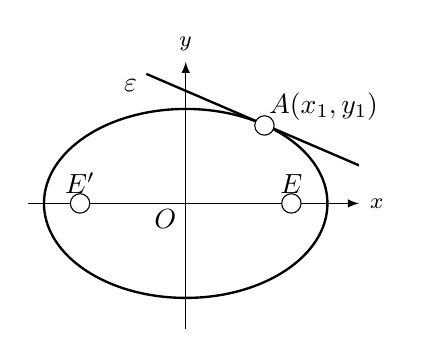
\begin{tikzpicture}
\begin{axis}[xmin=-2,xmax=2.2,ymin=-1.6,ymax=1.8,x=1cm,y=1cm,
ticks=none,xlabel={\footnotesize $ x $},ylabel={\footnotesize $ y $},
aks_on,belh ar]
\pgfmathsetmacro{\a}{1.8}
\pgfmathsetmacro{\b}{1.2}
\pgfmathsetmacro{\c}{sqrt(\a^2 - \b^2)}
\draw[pl](axis cs:0,0) ellipse (\a cm and \b cm);
\addplot [domain=-.5:2.8,\xrwma,pl] {-.43*x+1.43};
\coordinate (E) at (axis cs:\c, 0);
\coordinate (E') at (axis cs:-\c, 0);
\node (A) at (axis cs:1,.99) {};
\node at (axis cs:-.7,1.5){$\varepsilon$};
\end{axis}
\tkzLabelPoint[above](E){$E$}
\tkzLabelPoint[above right=-.9mm](A){$A(x_1,y_1)$}
\tkzLabelPoint[above](E'){$E'$}
\tkzDrawPoints[size=7,fill=white](E,E',A)
\node at (1.74,1.4) {$O$};
\end{tikzpicture}}{
Έστω $ A(x_1,y_1) $ το σημείο επαφής της εφαπτομένης με την έλλειψη. Τότε η εξίσωση της εφαπτομένης για κάθε μορφή έλλειψης από της παραπάνω είναι :
\begin{itemize}
\item Για την έλλειψη με εστίες στον άξονα $ x'x $ :  $ \displaystyle(\varepsilon) : \frac{xx_1}{a^2}+\frac{yy_1}{\beta^2}=1 $
\item Για την έλλειψη με εστίες στον άξονα $ y'y $ : $ \displaystyle (\varepsilon) : \frac{yy_1}{a^2}+\frac{xx_1}{\beta^2}=1 $
\end{itemize}}\mbox{}\\\\\\
\Orismos{Εκκεντρότητα Έλλειψησ}
Εκκεντρότητα μιας έλλειψης ονομάζεται ο θετικός πραγματικός αριθμός $ \varepsilon\in\mathbb{R}^+ $ που ορίζεται ο λόγος της εστιακής απόστασης προς το μήκος του μεγάλου της άξονα.
\[ \varepsilon=\dfrac{\gamma}{a} \]
H εκκεντρότητας μιας έλλειψης χαρακτηρίζει το σχήμα της. Όσο μεγαλύτερη εκκεντρότητα έχει μια έλλειψη, τόσο επιμήκης είναι κατα μήκος του μεγάλου της άξονα.
\begin{center}
\begin{tabular}{p{4.5cm}cp{4.5cm}}
\begin{tikzpicture}
\begin{axis}[
xmin=-2,xmax=2.2,ymin=-1.5,ymax=1.7,x=1cm,y=1cm,ticks=none,xlabel={$ x $},
ylabel={$ y $},aks_on,belh ar,
%scale only axis,unit vector ratio={2 1},
]
\pgfmathsetmacro{\a}{1.7}
\pgfmathsetmacro{\b}{1.3}
\pgfmathsetmacro{\c}{sqrt(\a^2 - \b^2)}
\draw[\xrwma!30,pl] (axis cs:0,0) ellipse (\a cm and \b cm);
\draw[\xrwma!50,pl] (axis cs:0,0) ellipse (\a cm and 0.75*\b cm);
\draw[\xrwma!70,pl] (axis cs:0,0) ellipse (\a cm and 0.5*\b cm);
\coordinate (E) at (axis cs:\c,0);
\coordinate (E') at (axis cs:-\c,0);
\coordinate (O) at (axis cs:0, 0);
\tkzLabelPoint[below](E){\footnotesize$E$}
\tkzLabelPoint[below](E'){\footnotesize$E'$}
\tkzLabelPoint[below left=1mm,fill=white,inner sep=.2mm](O){$O$}
\end{axis}
\draw[fill=\xrwma!30] (0.1,4) circle (.07) node[right]{\scriptsize{$\varepsilon=0.64$}};
\draw[fill=\xrwma!50] (1.5,4) circle (.07) node[right]{\scriptsize{$\varepsilon=0.81$}};
\draw[fill=\xrwma!70] (3,4) circle (.07) node[right]{\scriptsize{$\varepsilon=0.92$}};
\tkzDrawPoints(E,E')
\end{tikzpicture}	&  & 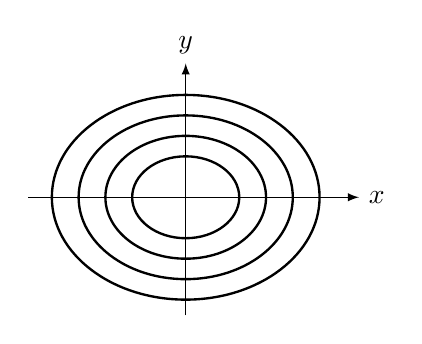
\begin{tikzpicture}
\begin{axis}[
xmin=-2,xmax=2.2,ymin=-1.5,ymax=1.7,x=1cm,y=1cm,ticks=none,xlabel={$ x $},
ylabel={$ y $},aks_on,belh ar,]
\pgfmathsetmacro{\a}{1.7}
\pgfmathsetmacro{\b}{1.3}
\pgfmathsetmacro{\c}{sqrt(\a^2 - \b^2)}
\draw[pl] (axis cs:0,0) ellipse (\a cm and \b cm);
\draw[pl] (axis cs:0,0) ellipse (0.8*\a cm and 0.8*\b cm);
\draw[pl] (axis cs:0,0) ellipse (0.6*\a cm and 0.6*\b cm);
\draw[pl] (axis cs:0,0) ellipse (0.4*\a cm and 0.4*\b cm);
\end{axis}
\end{tikzpicture} \\ 
\end{tabular} 
\end{center}
Οι ελλείψεις που έχουν την ίδια εκκεντρότητα ονομάζονται \textbf{όμοιες}.\\\\
\thewrhmata
\Thewrhma{Συμμετρικά σημεία}
Αν $ M(x,y) $ είναι ένα τυχαίο σημείο μιας έλλειψης με εξίσωση $ \frac{x^2}{a^2}+\frac{y^2}{\beta^2}=1 $ τότε τα συμμετρικά του σημεία :
 $ M_1(-x,y) $ ως προς τον άξονα $ y'y,\  M_2(-x,-y) $ ως προς την αρχή των αξόνων και $ M_3(x,-y) $ ως προς τον άξονα $ x'x $ ανήκουν κι αυτά στην καμπύλη της έλλειψης.
\begin{center}
\begin{tabular}{cc}
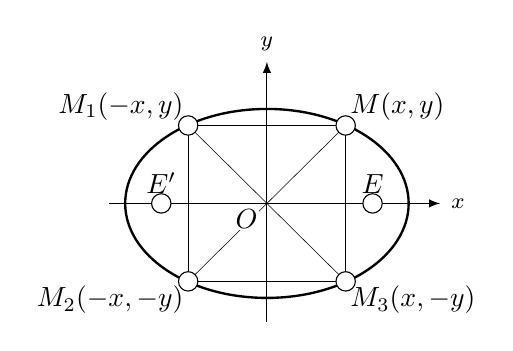
\begin{tikzpicture}
\begin{axis}[xmin=-2,xmax=2.2,ymin=-1.5,ymax=1.8,x=1cm,y=1cm,
ticks=none,xlabel={\footnotesize $ x $},ylabel={\footnotesize $ y $},
aks_on,belh ar]
\pgfmathsetmacro{\a}{1.8}
\pgfmathsetmacro{\b}{1.2}
\pgfmathsetmacro{\c}{sqrt(\a^2 - \b^2)}
\draw[pl](axis cs:0,0) ellipse (\a cm and \b cm);
\coordinate (E) at (axis cs:\c, 0);
\coordinate (E') at (axis cs:-\c, 0);
\node (A) at (axis cs:1,.99) {};
\node (B) at (axis cs:-1,.99) {};
\node (C) at (axis cs:-1,-.99) {};
\node (D) at (axis cs:1,-.99) {};
\end{axis}
\tkzDrawSegments(A,B B,C C,D D,A A,C B,D)
\tkzLabelPoint[above](E){$E$}
\tkzLabelPoint[above right=-.9mm](A){$M(x,y)$}
\tkzLabelPoint[above left=-.9mm](B){$M_1(-x,y)$}
\tkzLabelPoint[below left=-.9mm](C){$M_2(-x,-y)$}
\tkzLabelPoint[below right=-.9mm](D){$M_3(x,-y)$}
\tkzLabelPoint[above](E'){$E'$}
\tkzDrawPoints[size=7,fill=white](E,E',A,B,C,D)
\node[fill=white,inner sep=.2mm] at (1.74,1.3) {$O$};
\end{tikzpicture}
 & 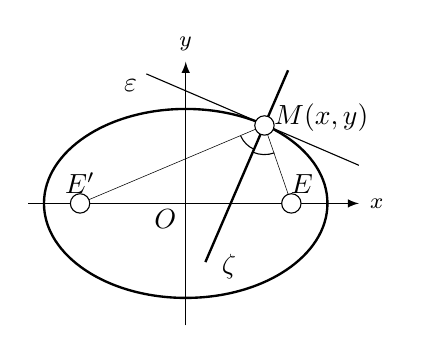
\begin{tikzpicture}
\begin{axis}[xmin=-2,xmax=2.2,ymin=-1.55,ymax=1.8,x=1cm,y=1cm,
ticks=none,xlabel={\footnotesize $ x $},ylabel={\footnotesize $ y $},
aks_on,belh ar]
\pgfmathsetmacro{\a}{1.8}
\pgfmathsetmacro{\b}{1.2}
\pgfmathsetmacro{\c}{sqrt(\a^2 - \b^2)}
\draw[pl](axis cs:0,0) ellipse (\a cm and \b cm);
\addplot [domain=-.5:2.8] {-.43*x+1.43};
\addplot [domain=.25:1.3,\xrwma,pl] {2.32*x-1.325};
\coordinate (E) at (axis cs:\c, 0);
\coordinate (E') at (axis cs:-\c, 0);
\node (A) at (axis cs:1,.99) {};
\node at (axis cs:-.7,1.5){$\varepsilon$};
\node at (axis cs:.55,-.8){$\zeta$};
\end{axis}
\draw (A)+(204:.33cm) arc (204:247:.33cm);
\draw (A)+(247:.37cm) arc (247:290:.37cm);
\tkzDrawSegments(E,A A,E')
\tkzLabelPoint[above right,xshift=-1.3mm](E){$E$}
\tkzLabelPoint[above right,yshift=-2mm](A){$M(x,y)$}
\tkzLabelPoint[above](E'){$E'$}
\tkzDrawPoints[size=7,fill=white](E,E',A)
\node at (1.74,1.35) {$O$};
\end{tikzpicture} \\ 
\end{tabular} 
\end{center}
\Thewrhma{Ανακλαστική Ιδιότητα}
Η ευθεία που διέρχεται από ένα τυχαίο σημείο $ M $ μιας έλλειψης και είναι κάθετη στην εφαπτόμενη ευθεία στο σημείο αυτό, διχοτομεί τη γωνία που σχηματίζουν τα ευθύγραμμα τμήματα που ενώνουν το σημείο με τις εστίες της έλλειψης.
\[ \zeta\hat{M}E=E'\hat{M}\zeta \]
Η ιδιότητα αυτή της έλλειψης ονομάζεται \textbf{ανακλαστική} και δείχνει οτι κάθε ευθεία γραμμή που διέρχεται από τη μια εστία της έλλειψης, ανακλάται πάνω στην έλλειψη με τέτοιο τρόπο ώστε η γωνία πρόσπτωσης να είναι ίση με τη γωνία ανάκλασης της με αποτέλεσμα να συναντήσει την άλλη εστία της έλλειψης. 
\end{document}
